
\noindent
\begin{tabular}{cc}
\begin{minipage}{0.60\textwidth}
\begin{exerciseS}[Giochi d'acqua]
Un getto d'acqua ($\rho=999\ kg/m^3 $) stazionario, piano e verticale 
viene indirizzato su un oggetto di massa $M$, tenuto da esso in equilibrio.
 Il getto ha distribuzione di velocità uniforme $U$ lungo lo spessore $H$, 
 mentre la distribuzione sul bordo dell'oggetto è 
triangolare di spessore $h$ con velocità massima $V$. Si calcoli la velocità $V$
e la massa $M$ dell'oggetto supponendo che:
\begin{itemize}
  \item il fluido che circonda il getto e il solido \`e aria in quiete a
  pressione atmosferica di $P_a = 101325\  Pa$;
  \item si possa trascurare la gravità nel bilancio di quantità di moto, ma non
nell'equilibrio del corpo.
\end{itemize} 


($V = U H / h ; M = \rho U^2 H / g$)
\end{exerciseS}
\end{minipage}
&
\begin{minipage}{0.35\textwidth}
   \begin{center}
   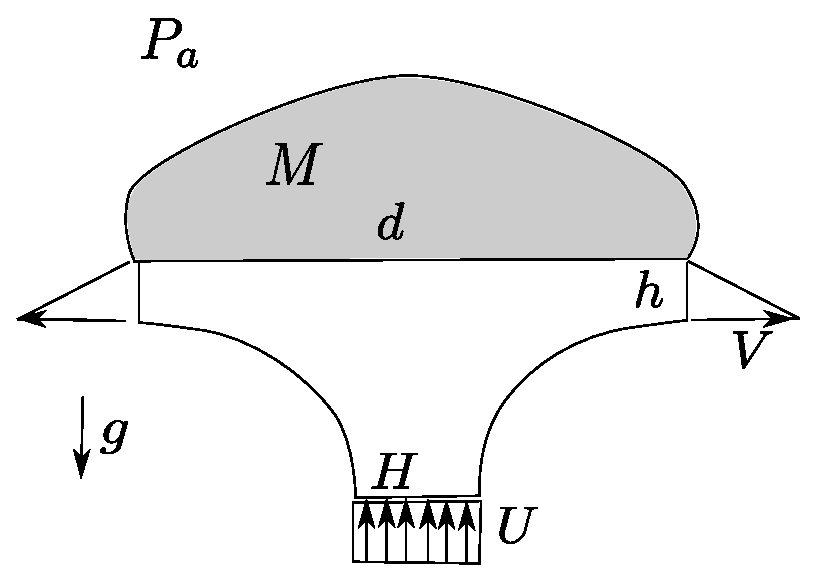
\includegraphics[width=0.90\textwidth]{./fig/gettoPiattello.eps}
   \end{center}
\end{minipage}
\end{tabular}

\vspace{1.0cm}

\sol

\partone
  Bilanci integrali di massa e quantità di moto. Equazioni di equilibrio (equazioni fondamentali della dinamica classica). Principio di azione e reazione. Integrale della normale su una superficie chiusa è identicamente nullo.

\parttwo
 Ipotesi: problema stazionario; sulla superficie libera del corpo e del fluido agisce solo la pressione ambiente $p_a$; nessun effetto della gravità nei bilanci del fluido.

Si sceglie un asse $y$ diretto verso l'alto.

\begin{itemize}
 \item Scrittura delle equazioni di bilancio per il fluido.
 
   \begin{equation}
     \begin{cases}
       \frac{d}{d t} \int_{\Omega} \rho + \oint_{\partial \Omega} \rho \bm{u} \cdot \hat{\bm{n}} = 0 & \qquad \text{(massa)} \\
       \frac{d}{d t} \int_{\Omega} \rho \bm{u} + \oint_{\partial \Omega} \rho \bm{u} \bm{u} \cdot \hat{\bm{n}} +
        \oint_{\partial \Omega} p \hat{\bm{n}} - \oint_{\partial \Omega} \bm{s_n} 
        -\int_V \rho \bm{g} = 0  
        & \qquad \text{(quantità di moto)}  %\Rb^{ext}
      \end{cases}
    \end{equation}

A queste, va aggiunta l'equazione di equilibrio del corpo sottoposto alla forza di gravità: $\bm{F} + M \bm {g} = 0$.

\item Dopo aver semplificato il bilancio di massa, da esso si ricava la velocità $V$. La velocità
 sui due
bordi 'di uscita' è $v(s) = V s/h$, avendo chiamato $s$ la coordinata che descrive tale superficie per valori compresi tra $0$ e $h$.
\begin{equation}
  0 = \int_{S_in} \rho \bm{u} \cdot \bm{\hat{n}} +   \int_{S_{out1}} \rho \bm{u} \cdot \bm{\hat{n}} +
  \int_{S_{out2}} \rho \bm{u} \cdot \bm{\hat{n}} = 
  - \rho U H + 2 \int_0^h \rho V \frac{s}{h} ds = \rho \displaystyle\left[
- U H + 2 \frac{1}{2} V h\right]
\end{equation}

E quindi $V = U \frac{H}{h}$.

 \item Le equazioni vengono opportunamente semplificate secondo le ipotesi fatte (vengono eliminati i termini non stazionari e il termine contenente le forze di volume - gravità). Il bordo del dominio fluido $\partial \Omega$ viene indicato con $S_f$. I contributi di pressione e viscosi vengono raccolti nel "vettore di sforzo" complessivo.


 
\begin{equation}
\begin{split}
% & \Rb = \oint_{S_{s}}  {\bm{t}}_{\bm{n}} = 
% \oint_{S_{s}}  {\bm{s}}_{\bm{n}} - \oint_{S_{s}} p {\hat{\bm{n}}}_{s} \\
 & \oint_{S_f} \rho \bm{u} \bm{u} \cdot \hat{\bm{n}}= 
 \oint_{S_{f}}  {\bm{s}}_{\bm{n}} - \oint_{S_f} p {\hat{\bm{n}}}
  = \oint_{S_{f}}  {\bm{t}}_{\bm{n}} 
\end{split}
\end{equation}


%\begin{equation}
%  \Rb = \oint_{S_{s}} \bm{t_n} = 
%  \int_{S_{ext}} \bm{t_n} + \int_{S_{c}} \bm{t_n} = 
%  - \int_{S_{ext}} p \bm{n}_{s} + \int_{S_{c}} \bm{t_n} = 
%\end{equation}


\item Riscrittura del termine di contorno. Si indica con $S_f$ il contorno fluido: questo è costituito dall'unione del controno a contatto con il corpo $S_c$ e quella "libera" $S_l$. Il contorno del corpo $S_{s}$ è suddiviso nel contorno $S_c$ a contatto con il fluido e nel contorno libero $S_{c_l}$.

Nei passaggi successivi si ricava il legame tra sforzi sul contorno del dominio fluido e la forza agente sul corpo.
Si usano le ipotesi che sulle superfici libere agisca solo la pressione ambiente. Si usa il fatto che l'integrale di una quantità costante per la normale su una superficie chiusa è nullo. Vengono
definite le normali $\bm{n}$ e $\bm{n_s}$ come la normale uscente dal volume del fluido e quella
uscente dal solido. Si definiscono $\bm{t}_{\bm{n}}$ e $\bm{t}_{\bm{n}_{s}}$ come lo sforzo agente sul fluido e quello agente sul solido. Si usa infine il fatto che $\bm{n}=-\bm{n}_{s}$ (normali uscenti dai due domini, uguali e contrarie) e
$\bm{t_n}=-\bm{t}_{\bm{n}_s}$ sulla superficie in comune (sforzi agenti sulla superficie comune, uguali e contrari; principio di azione e reazione).

\begin{equation}
\begin{aligned}
  \oint_{S_f} \bm{t_n} & = 
  \int_{S_l} \bm{t_n} + \int_{S_c} \bm{t_n} = & \text{($\bm{t_n} |_{S_l} = -p_a \bm{n}$ )}\\
  & = - \int_{S_l} p_a \bm{n} + \int_{S_c} \bm{t_n} = & \text{(somma e sottrazione di $\int_{S_c} p_a \bm{n}$)}\\
  & = \underbrace{- \int_{S_l} p_a \bm{n} - \int_{S_c} p_a \bm{n}}_{=0}
  + \int_{S_c} p_a \bm{n} + \int_{S_c} \bm{t_n} = & \text{($\bm{n} = -\bm{n}_{s}$)} \\
  & = - \int_{S_c} p_a \bm{n}_{s} + \int_{S_c} \bm{t_n} = &
  \text{($S_{s} = S_c \cup S_{c_l}$ e $\int_{S_{s}} p_a \bm{n} = 0$)}\\
  & = \int_{{S_c}_l} p_a \bm{n}_{s} + \int_{S_c} \bm{t_n} = &
  \text{($\bm{t}_{\bm{n}_{s}}|_{S_{c_l}} = -p_a \bm{n}_{s}$, $\bm{t}_{\bm{n}_{s}}|_{S_c} = - \bm{t_n}$)} \\
  & = - \int_{{S_c}_l} \bm{t}_{\bm{n}_{s}} - \int_{S_c} \bm{t}_{\bm{n}_{s}} = \\
  & = - \int_{S_{s}} \bm{t}_{\bm{n}_{s}} \\
  & = - \bm{R}
\end{aligned}
\end{equation}
% \item Riscrittura integrali di contorno % della pressione
%
%\begin{equation}
%\begin{split}
%  & \oint_{S_{s}} p {\hat{\bm{n}}}_{s} = 
%   \int_{S_c} (p-p_0) {\hat{\bm{n}}}_{s}
%   + \oint_{S_{s}} p_0 {\hat{\bm{n}}}_{s} =
%   \int_{S_c} (p-p_0) {\hat{\bm{n}}}_{s} \\
%  & \oint_{S_{f}} p {\hat{\bm{n}}} = 
%   \int_{S_c} (p-p_0) {\hat{\bm{n}}}
%   + \oint_{S_{f}} p_0 {\hat{\bm{n}}} =
%   \int_{S_c} (p-p_0) {\hat{\bm{n}}} = - \int_{S_c} (p-p_0) {\hat{\bm{n}}}_{s}\\   
%\end{split}
%\end{equation}


%\item Le relazioni semplificate vengono inserite nelle equazioni di equilibrio; si può scrivere quindi:
%\begin{equation}
%\begin{split}
%  \Rb & = - \oint_{S_{s}} p {\hat{\bm{n}}}_{s} = 
%   - \oint_{S_{c}} (p-p_0) {\hat{\bm{n}}}_{s} = 
%   \oint_{S_{c}} (p-p_0) {\hat{\bm{n}}} = 
%   -\oint_{S_f} \rho \bm{u} \bm{u} \cdot \hat{\bm{n}}
%\end{split}
%\end{equation}

\item Sostituendo nell'equazione del bilancio della quantità di moto si ottiene:
\begin{equation}
  \bm{R} = - \oint_{S_f} \rho \bm{u} \bm{u} \cdot \hat{\bm{n}} 
\end{equation}

\item Data la simmetria del problema si riconosce che non ci può essere una componente orizzontale.
I contributi nel bilancio della quantità di moto sulla superficie di contatto tra corpo e fluido e 
sulla superficie laterale del getto sono nulli poichè è nullo il flusso su tali superfici.
I contributi sulle sezioni 'di uscita' sono uguali e contrari. Rimane quindi solo il contributo 
dalla sezione 'in ingresso'.

\begin{equation}
  \bm{F} = - \oint_{S_f} \rho \bm{u} \bm{u} \cdot \bm{\hat{n}} = 
           - \oint_{S_in} \rho \bm{u} \bm{u} \cdot \bm{\hat{n}} = 
           \rho U^2 H \bm{\hat{y}}
\end{equation}

\item Si scrive l'equilibrio del corpo $\bm{F} + M \bm{g} = 0$, con $\bm{g} = - g \bm{\hat{y}}$.
Da questo segue che $M = F/g = \frac{\rho U^2 H}{g}$.

\end{itemize}


\textit{Osservazioni.} 
Nell'elaborazione dei termini della quantità di moto è contenuta la forma della risultante delle forze sull'oggetto vista in classe.

Come giustamente osservato da qualcuno in classe, la massa è per unità di lunghezza, poichè stiamo considerando un caso bidimensionale.
